
\section{Rappresentazione geometrica del sistema}
Prima di definire le strategie di gestione della sicurezza, è necessario introdurre una rappresentazione geometrica del robot e dell'operatore che possa essere impiegata per effettuare le verifiche di prossimità in tempo reale. La geometria reale di un manipolatore e del corpo umano è infatti complessa e una sua modellazione dettagliata risulterebbe computazionalmente troppo onerosa per i calcoli da eseguire continuamente durante il movimento. Per questo motivo, entrambi vengono approssimati mediante volumi geometrici semplificati (primitive geometriche).

\subsection{Sphere Swept Lines (SSL)}

Una delle rappresentazioni più diffuse per questo scopo è costituita dalle \textit{Sphere Swept Lines} (SSL), le quali permettono di approssimare la geometria di un corpo tramite l'unione di un segmento e di una sfera. Nel caso di un segmento di estremi $P_0$ e $P_1$, la SSL corrispondente è definita formalmente come la somma di Minkowski tra il segmento $\overline{P_0P_1}$ e una sfera di raggio $r$ \cite{larsen1999fast}.

In generale, dati due insiemi $A$ e $B$ nello spazio euclideo, la loro somma di Minkowski è definita come:
\begin{equation}
    A+B = \{a+b \mid a\in A,\; b\in B\}.
\end{equation}

Nel caso specifico delle SSL, la somma di Minkowski tra il segmento e la sfera genera un solido a forma di capsula, interpretabile come il luogo dei punti nello spazio aventi distanza minore o uguale a $r$ dal segmento $\overline{P_0P_1}$.

\begin{figure}[htbp]
    \centering
    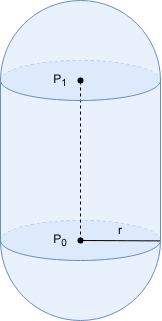
\includegraphics[width=0.2\linewidth]{figure_tesi/SSL.png}
    \caption{Rappresentazione geometrica di una Sphere Swept Line (SSL).}
    \label{fig:SSL}
\end{figure}

L'impiego delle SSL consente quindi di sostituire una geometrie tridimensionali articolate con un insieme contenuto di primitive, semplificando notevolemnte il calcolo algebrico delle distanze minime e l'individuazione di eventuali intersezioni tra robot e operatore.

\subsection{Modellazione del robot e dell'operatore}

Nel presente lavoro, il robot utilizzato per le prove sperimentali è un manipolatore Franka Emika Panda a sette gradi di libertà. Ai fini della valutazione della distanza dall'operatore, la struttura del robot viene approssimata tramite un insieme di quattro SSL (capsule), associate rispettivamente alle coppe di giunti principali: base-1, 2-3, 4-5, 6-flangia. In figura \ref{fig:robot_modellazione} si può osservare 

I segmenti delle capsule vengono definiti in tempo reale a partire dalla cinematica diretta del robot, quindi dalle posizioni dei giunti, mentre il raggio $r$ di ciascuna SSL viene opportunamente dimensionato in modo da racchiudere interamente il volume del braccio robotico nel tratto corrispondente. L'aggiornamento continuo della posizione dei giunti durante il moto permette di ricalcolare istante per istante la posa delle SSL, consentendo quindi di effettuare le verifiche di sicurezza in tempo reale.

\begin{figure}[htbp]
    \centering
    \begin{subfigure}[b]{1\textwidth}
        \centering
        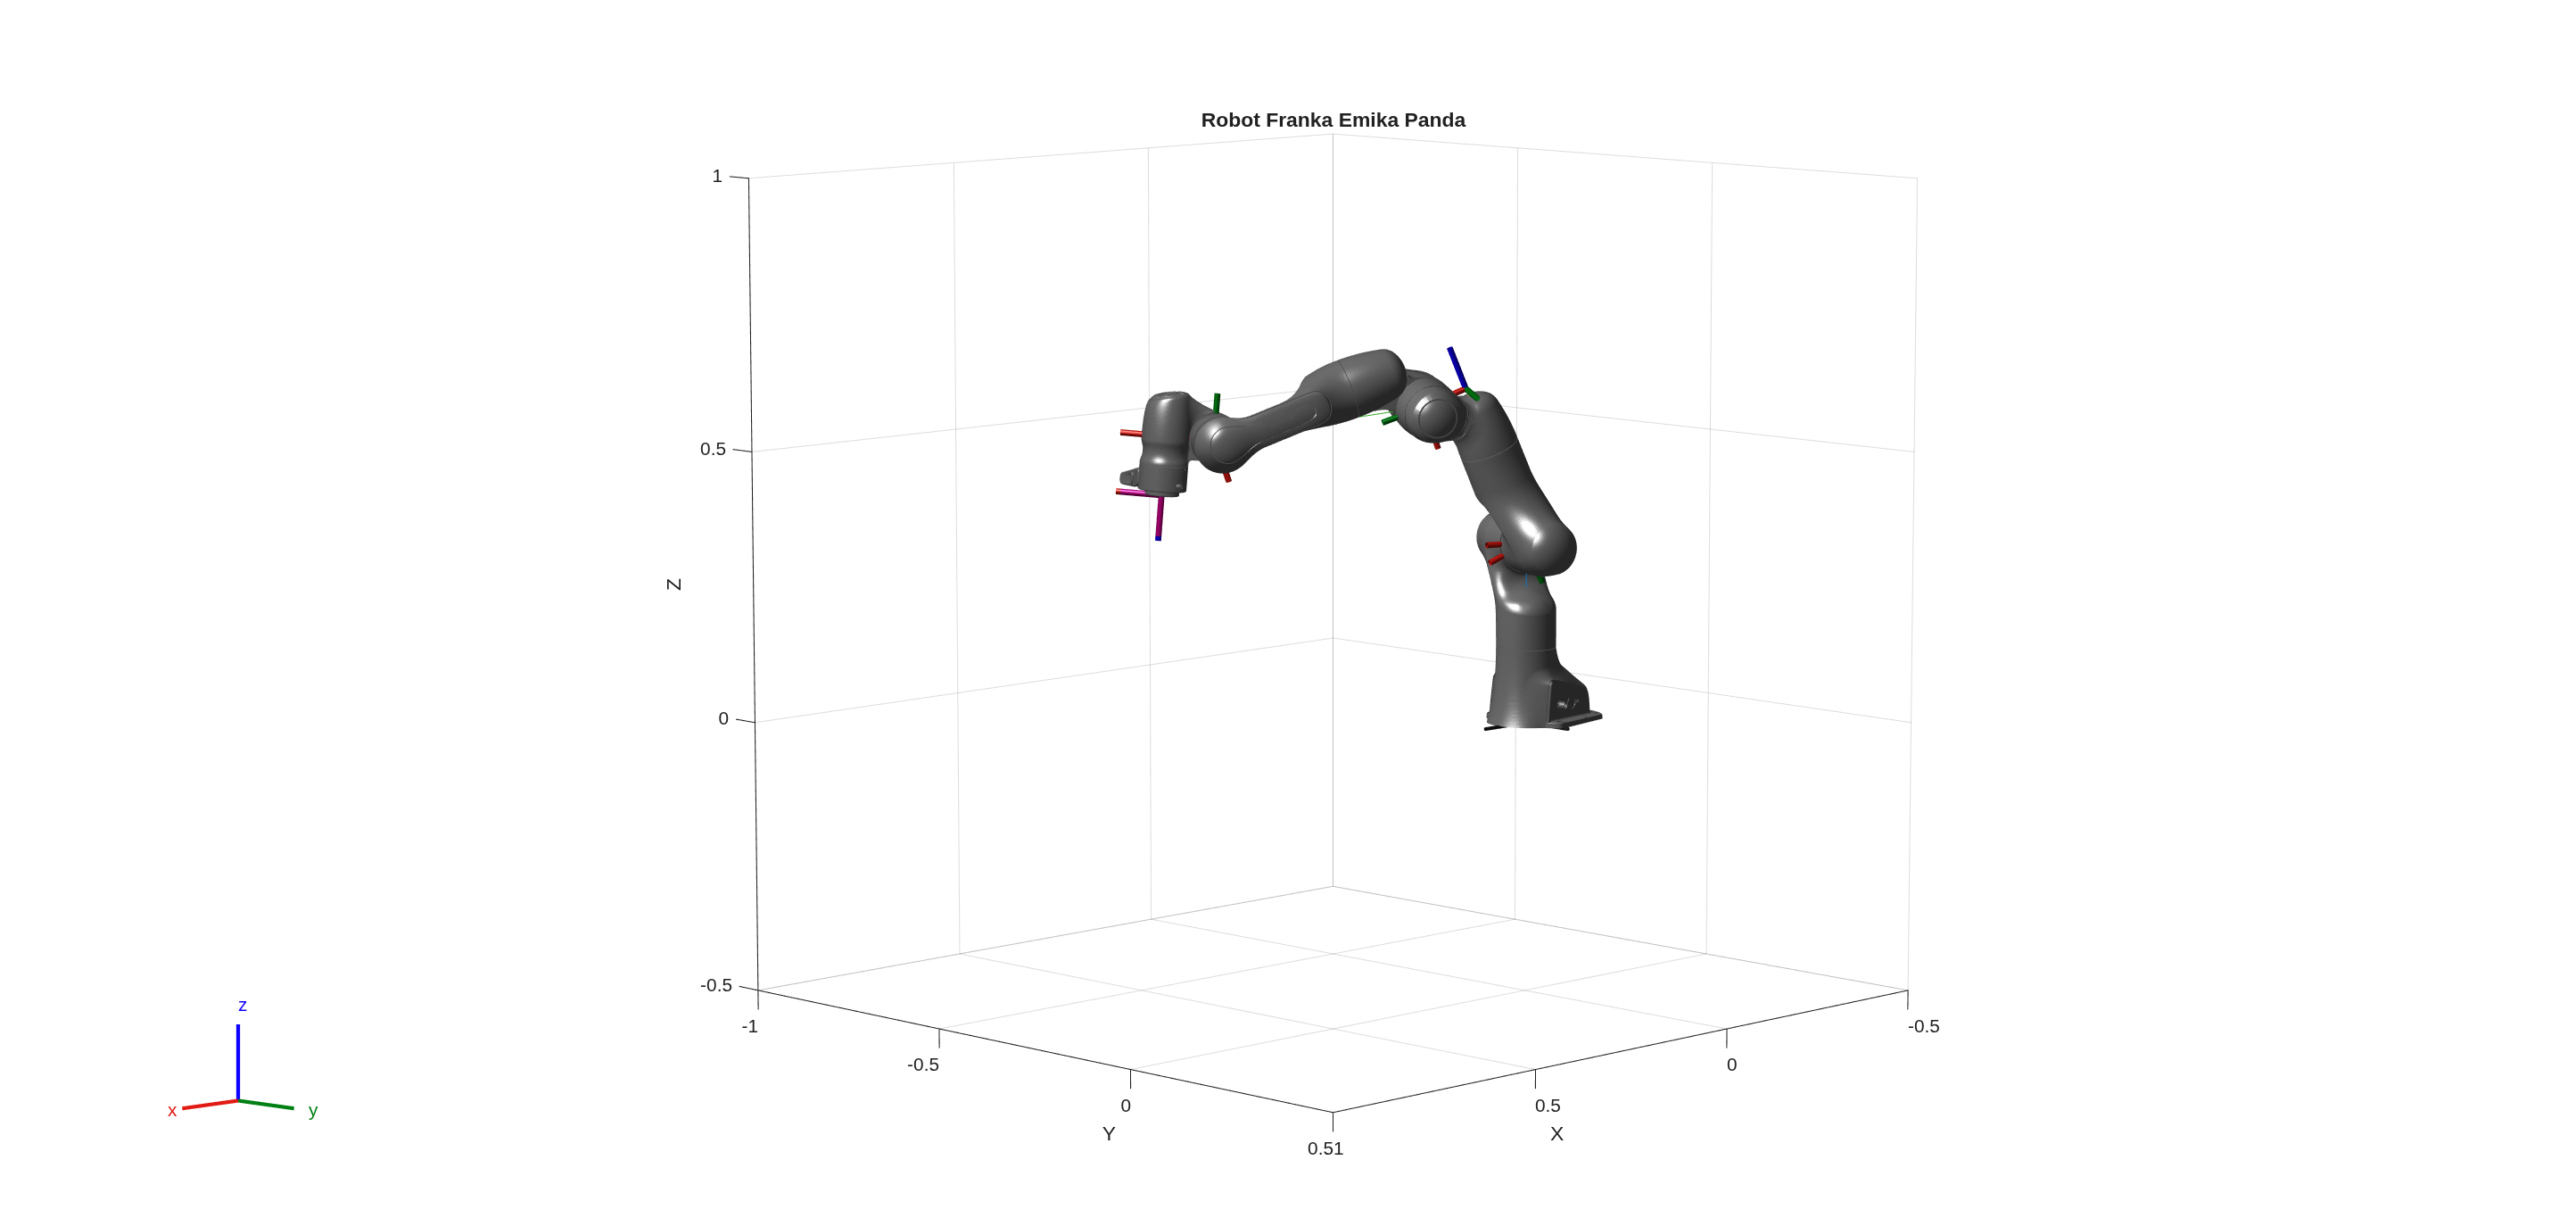
\includegraphics[width=\textwidth]{figure_tesi/robot.png}
        \caption{Robot Panda nella configurazione iniziale}
        \label{fig:robot}
    \end{subfigure}
    \hfill
    \begin{subfigure}[b]{1\textwidth}
        \centering
        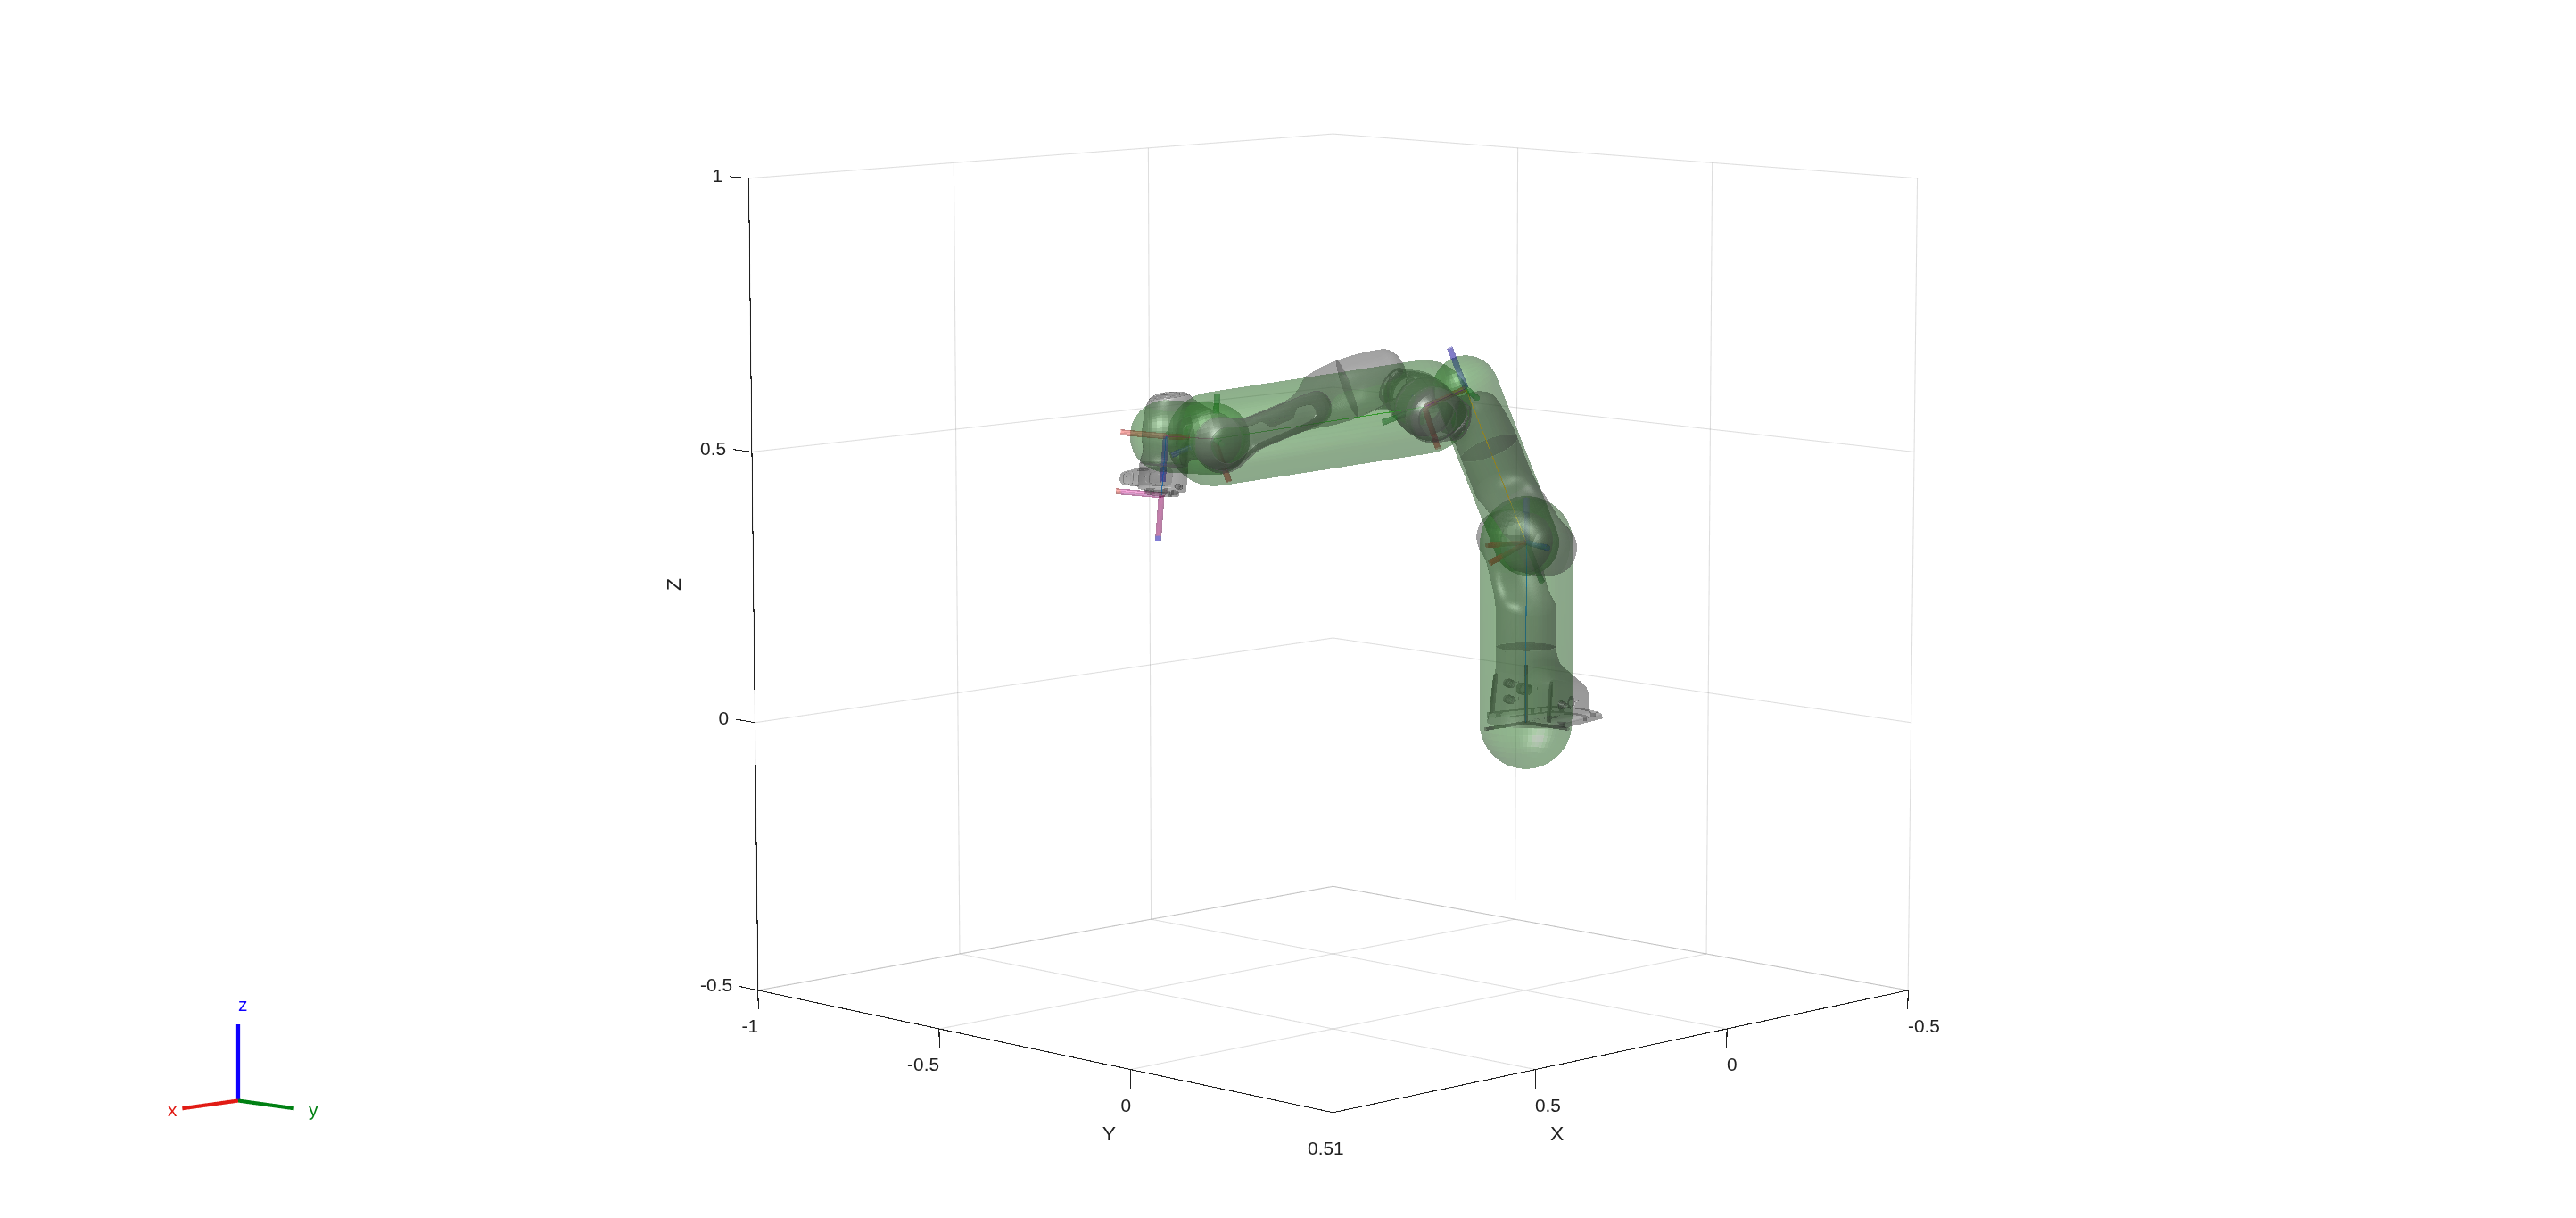
\includegraphics[width=\textwidth]{figure_tesi/robot_capsule.png}
        \caption{Modellazione geometrica tramite SSL}
        \label{fig:robot_capsule}
    \end{subfigure}
    \caption{Confronto tra la geometria dettagliata del robot (a) e la sua rappresentazione semplificata a capsule (b).} 
    \label{fig:robot_modellazione}
\end{figure}

In modo analogo, l'operatore umano viene modellato attraverso una scomposizione geometrica basata sullo scheletro tridimensionale rilevato dal sistema di visione. Tramite opportuni algoritmi di \textit{skeleton tracking} viene fornito un insieme ordinato di punti 3D corrispondenti alle principali articolazioni anatomiche (testa, spalle, gomiti, polsi, anche). Tali punti vengono utilizzati come estremi dei segmenti su cui vengono definite le SSL associate alle diverse parti del corpo dell'operatore.

\section{Distanza geometrica tra robot e operatore}

Come introdotto nella sezione precedente, sia il robot che l'operatore umano vengono approssimati tramite insiemi di primitive geometriche a capsula (SSL). Di conseguenza, la determinazione della distanza minima di sicurezza si riconduce al problema geometrico del calcolo della distanza minima tra i segmenti nello spazio tridimensionale $\mathbb{R}^3$, a cui viene successivamente sottratta la somma dei rispettivi raggi.

Si considerino due segmenti $S_1$ e $S_2$, individuati dalle rispettive coppie di estremi $(P_1, Q_1)$ e $(P_2, Q_2)$. Qualsiasi punto appartenente alle rette su cui giacciono tali segmenti può essere espresso in forma parametrica come:
\begin{align}
    \pmb{L_1(s)} &= \pmb{P_1} + s\pmb{D_1}, \quad \text{con } \pmb{D_1} = \pmb{Q_1} - \pmb{P_1} \\
    \pmb{L_2(t)} &= \pmb{P_2} + t\pmb{D_2}, \quad \text{con } \pmb{D_2} = \pmb{Q_2} - \pmb{P_2}
\end{align}
dove $s, t \in \mathbb{R}$ sono i parametri di linea. I punti appartengono ai segmenti fisici $S_1$ e $S_2$ se e solo se i rispettivi parametri soddisfano i vincoli $s \in [0,1]$ e $t \in [0, 1]$.

Definito il vettore di connessione tra le origini dei due segmenti $\pmb{R} = \pmb{P_1} - \pmb{P_2}$, il vettore che unisce due punti generici sulle due rette è espresso da:
\begin{equation}
    \pmb{v}(s,t) = L_1(s) - L_2(t) = \pmb{R} + s\pmb{D_1} - t\pmb{D_2}.
\end{equation}

Il problema di minima distanza equivale a minimizzare la norma al quadrato $||\pmb{v}(s,t)||^2$. Impostando le condizioni di ortogonalità del segmento di minima distanza rispetto alle direzioni dei due segmenti, ovvero $\pmb{v} \cdot \pmb{D_1} = 0$ e $\pmb{v} \cdot \pmb{D_2} = 0$, si ottiene un sistema di equazioni lineari il cui annullamento fornisce i valori ottimi dei parametri per le rette non parallele:
\begin{equation}
    s = \frac{(\pmb{D_1} \cdot \pmb{D_2})(\pmb{D_2} \cdot \pmb{R}) - (\pmb{D_2} \cdot \pmb{D_2})(\pmb{D_1} \cdot \pmb{R})}{(\pmb{D_1} \cdot \pmb{D_1})(\pmb{D_2} \cdot \pmb{D_2}) - (\pmb{D_1} \cdot \pmb{D_2})^2}
\end{equation}
\begin{equation}
    t = \frac{(\pmb{D_1} \cdot \pmb{D_1})(\pmb{D_2} \cdot \pmb{R}) - (\pmb{D_1} \cdot \pmb{D_2})(\pmb{D_1} \cdot \pmb{R})}{(\pmb{D_1} \cdot \pmb{D_1})(\pmb{D_2} \cdot \pmb{D_2}) - (\pmb{D_1} \cdot \pmb{D_2})^2}
\end{equation}

Qualora i valori di $s$ e $t$ così calcolati rientrino entrambi nell'intervallo $[0,1]$, i punti di minima distanza $C_1$ e $C_2$ si trivano all'interno dei segmenti e sono definiti da:
\begin{align}
    C_1 &= L_1(s) = \pmb{P_1} + s\pmb{D_1} \\
    C_2 &= L_2(t) = \pmb{P_2} + t\pmb{D_2}
\end{align}

Nel caso in cui uno o entrambi i parametri giacciano all'esterno dell'intervallo $[0,1]$, i punti di minima distanza si trovano sui bordi di almeno uno dei due segmenti. In tale eventualità, si satura il parametro fuori limite all'estremo più vicino, cioè $0$ o $1$, e si ricalcola analiticamente il valore dell'altro parametro mediante proiezione ortogonale sul relativo segmento, garantendo così il rispetto dei vincoli geometrici.

Come mostrato in Figura \ref{fig:distanze_segmenti}, trovati i due punti di minima distanza $C_1$ e $C_2$, la distanza euclidea tra i segmenti centrali risulta:
\begin{equation}
    d_{\text{seg}} = ||C_1 - C_2||
\end{equation}

In conclusione, la distanza effettiva $d_{\text{SSL}}$ tra le due primitive geometriche a capsula, caratterizzate dai rispettivi raggi $r_1$ e $r_2$, è ricavata sottraendo i due raggi dei volumi di ingombro:
\begin{equation}
    d_{\text{SSL}} = \max(0, \; d_{text{seg}} - r_1 -r_2)
\end{equation}

\begin{figure}
    \centering
    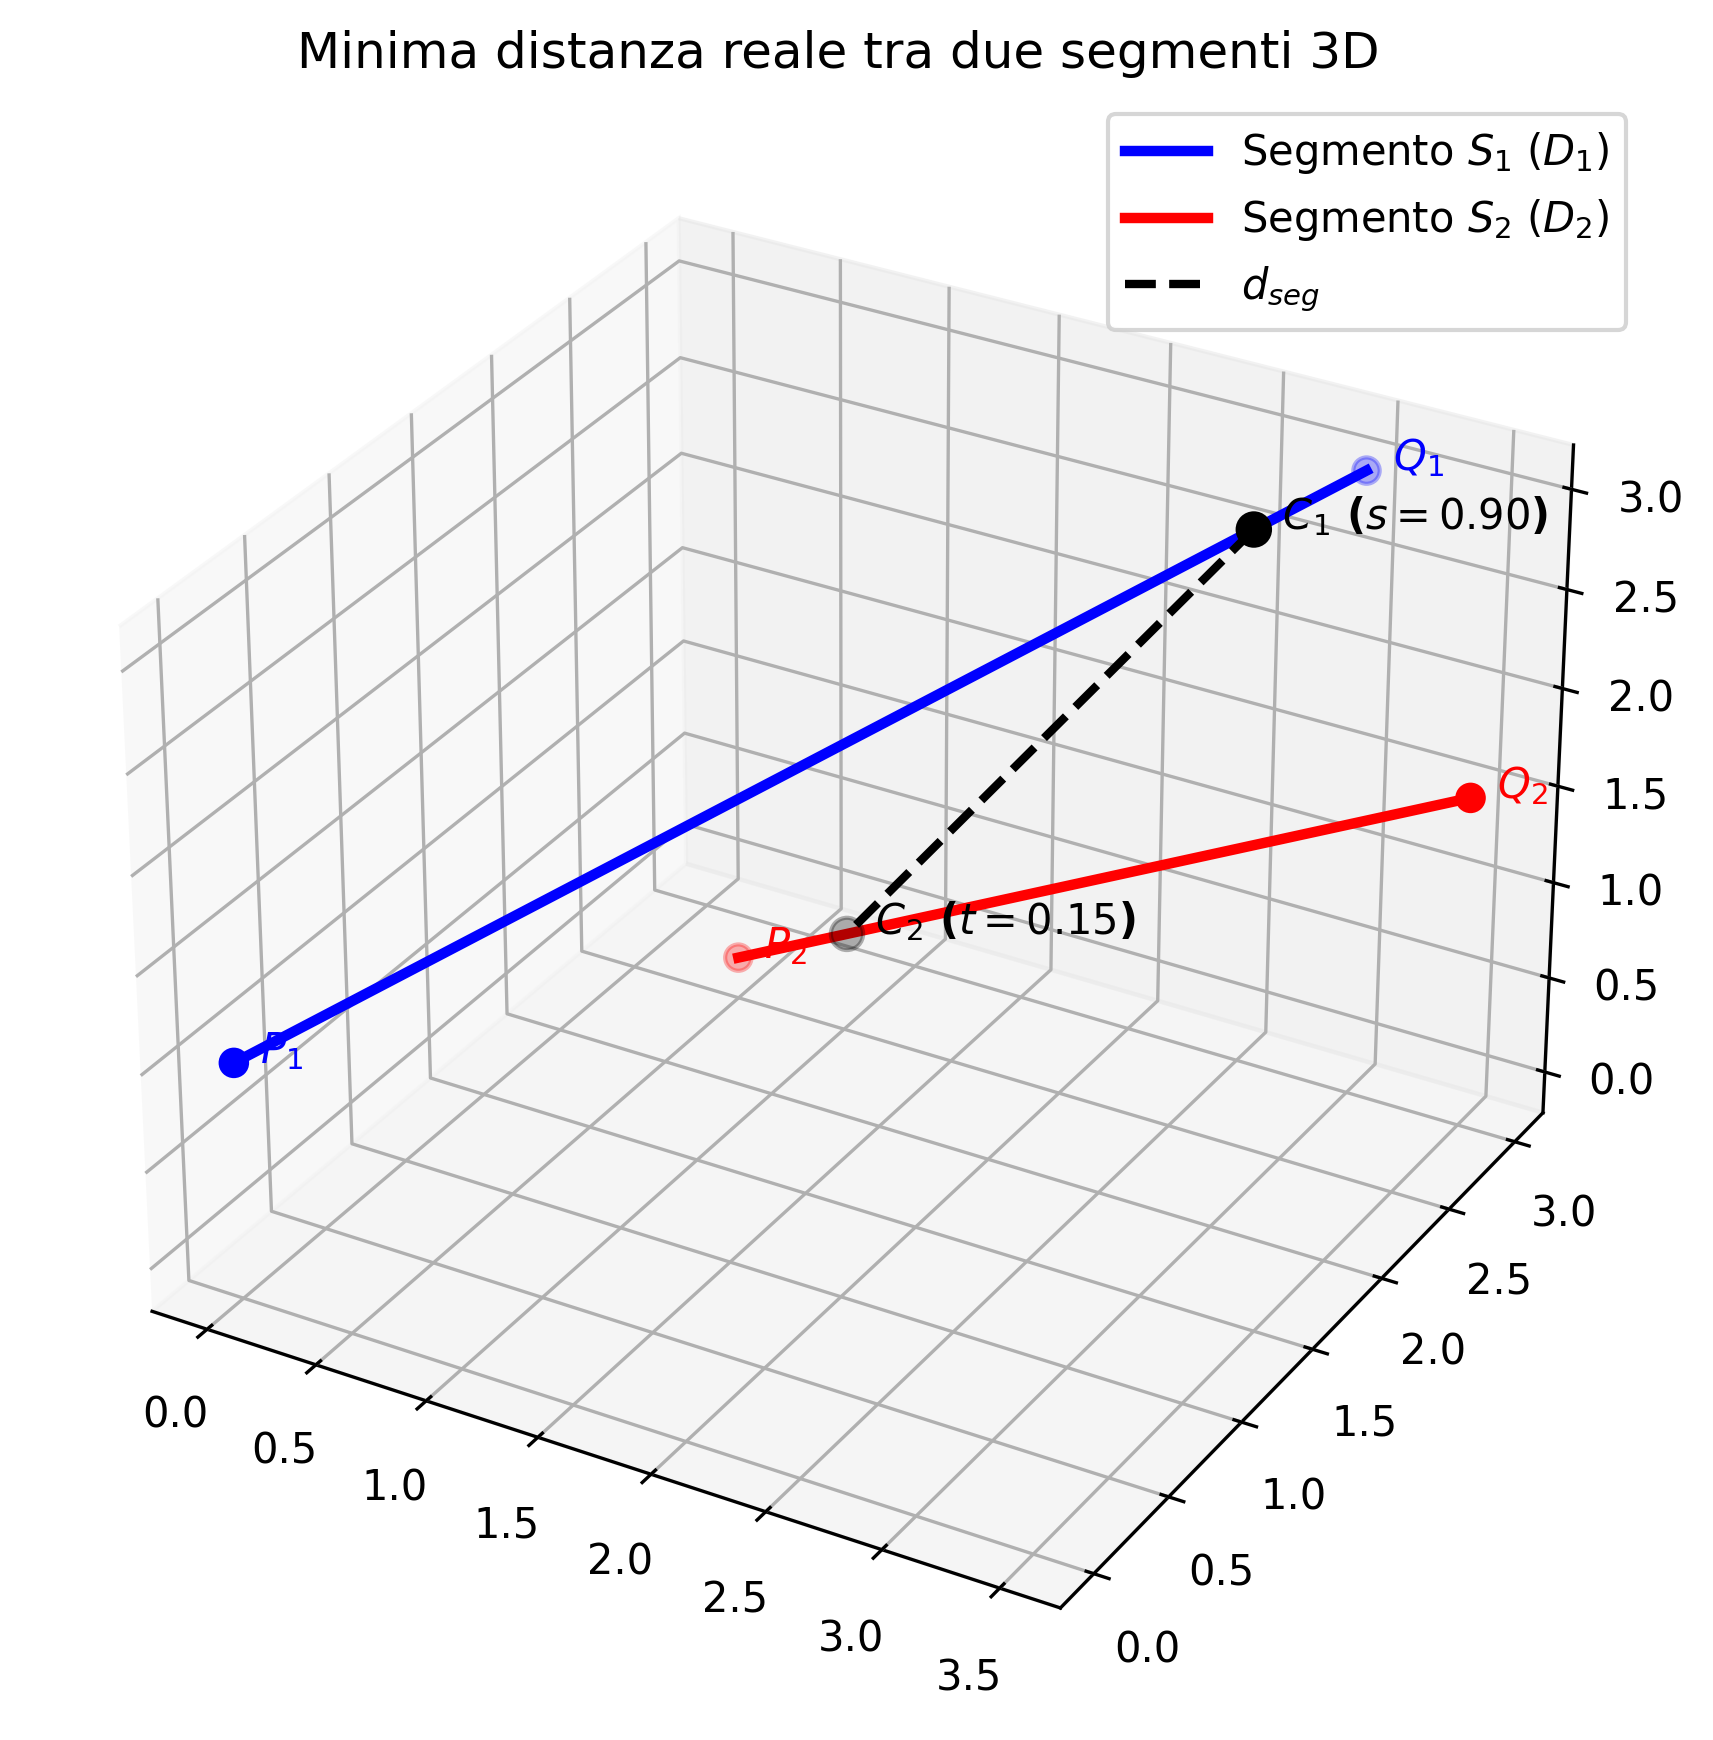
\includegraphics[width=0.5\linewidth]{figure_tesi/distanza_segmenti_corretta.png}
    \caption{Rappresentazione geometrica della distanza minima $d_{seg}$ tra due segmenti $S_1$ e $S_2$.}
    \label{fig:distanze_segmenti}
\end{figure}

\section{Primo approccio: dimensionamento dinamico delle zone di sicurezza}
\label{sec:primo_approccio}

Questo approccio alla collaborazione uomo-robot in sicurezza si basa sul principio di \textit{Speed and Separation Monitoring} (SSM). Per superare la rigidità dei metodi convenzionali con zone di sicurezza fisse o sovradimensionate, il sistema ottimizza online il tempo di arresto $T_{\text{stop}}$. 

\subsection{Principio dello Speed and Separation Monitoring (SSM)}
Secondo le direttive della specifica tecinca ISO/TS 15066 \cite{ISO15066}, la modalità di collaborazione SSM impone che la velocità operativa del manipolatore sia continuamente regolata in funzione della distanza relativa dall'operatore umano. L'obiettivo principale è garantire che la distanza di separazione corrente $S(t)$ tra qualsiasi punto del robot e l'operatore non sia mai inferiore a una distanza di sicurezza minima $S_{\text{min}}(t)$, definita come:
\begin{equation}
    S_{\text{min}}(t) = S_h(t) + S_r(t) + S_s(t) + C + Z_d + Z_r
    \label{eq:iso_ssm_distance}
\end{equation}
dove:
\begin{itemize}
    \item $S_h(t)$ rappresenta lo spostamento potenziale dell'operatore verso il robot durante la fase di reazione ed esecuzione dell'arresto;
    \item $S_r(t)$ è lo spazio percorso dal robot durante il tempo di reazione del sistema di controllo $t_r$;
    \item $S_s(t)$ rappresenta lo spazio effettivo di frenata del manipolatore;
    \item $C$, $Z_d$ e $Z_r$ sono termini cautelativi legati rispettivamente alle capacità di intrusione dell'operatore, alle incertezze dei sensori di tracciamento e alla tolleranza di posizionamento del robot.
\end{itemize}

Nei sistemi tradizionali, le componenti $S_s(t)$ e $S_r(t)$ vengono calcolate assumendo le peggiori condizioni cinematiche e dinamiche possibili (es. massima velocità e carico nominale), conducendo a distanze $S_{\text{min}}$ costanti, conservative e fortemente penalizzanti per la produttività. Per superare tale rigidità, il metodo qui descritto propone un'ottimizzazione in tempo reale del tempo di arresto $T_{\text{stop}}$, consentendo la generazione di capsule protettive dinamiche e adeguate all'effettivo stato cinematico del robot. La stima accurata di $T_{\text{stop}}$ consente di determinare l'effettivo spazio di frenata e di ridimensionare dinamicamente le capsule di sicurezza protettive, modellate come \textit{Sphere Swept Lines} (SSL), attorno ai bracci del manipolatore.

\subsection{Pianificazione online della traiettoria di arresto}
\label{subsec:traiettoria_stop}
Al momento della rilevazione di un potenziale rischio di collisione al generico istante temporale $t_0$, il controllore non applica un'interruzione discontinua della traiettoria nominale. Viene invece generata online una traiettoria di arresto continua e differenziabile del dominio dei giunti per evitare sollecitazioni impulsive sui riduttori. 

Si definisce $t_r$ il tempo di reazione dell'architettura di controllo. la manovra di frenata s sviluppa nell'intervallo temporale $t \in [t_i, t_f]$ dove $t_i = t_0 + t_r$ rappresenta l'istante di innesco reale della frenata e $t_f = t_0+t_r+T_{\text{stop}}$ specifica l'istante di arresto completo \cite{Scalera2024}.

Per imporre la continuità di posizione, velocità e accelerazione, la traiettoria di arresto $q_j(t)$, per $j = 1, \dots, 7$, viene descritta tramite un polinomio del $5^\circ$ grado \cite{Scalera2024}, per ciascuno dei $7$ giunti del manipolatore, :
\begin{equation}
    q_j(t) = a_0+a_1t+a_2t^2+a_3t^3+a_4t^4+a_5t^5
\end{equation}

I coefficienti $a_k$, per $k = 0, \dots, 5$, del polinomio vengono determinati analiticamente in tempo reale imponendo le condizioni al contorno tra lo stato cinematico iniziale di frenata al tempo $t_i$ e lo stato di arresto completo al tempo $t_f$:
\begin{equation}
    \begin{cases}
        q_j(t_i)=q_{i,j}, & q_j(t_f)=q_{i,j} \\
        \dot{q}_j(t_i)= \dot{q}_{i,j}, & \dot{q}_j(t_f) = 0 \\
        \ddot{q}_j(t_i) = \ddot{q}_{i,j}, & \ddot{q}_j(t_f) = 0
    \end{cases}
\end{equation}

\begin{figure}[htbp]
    \centering
    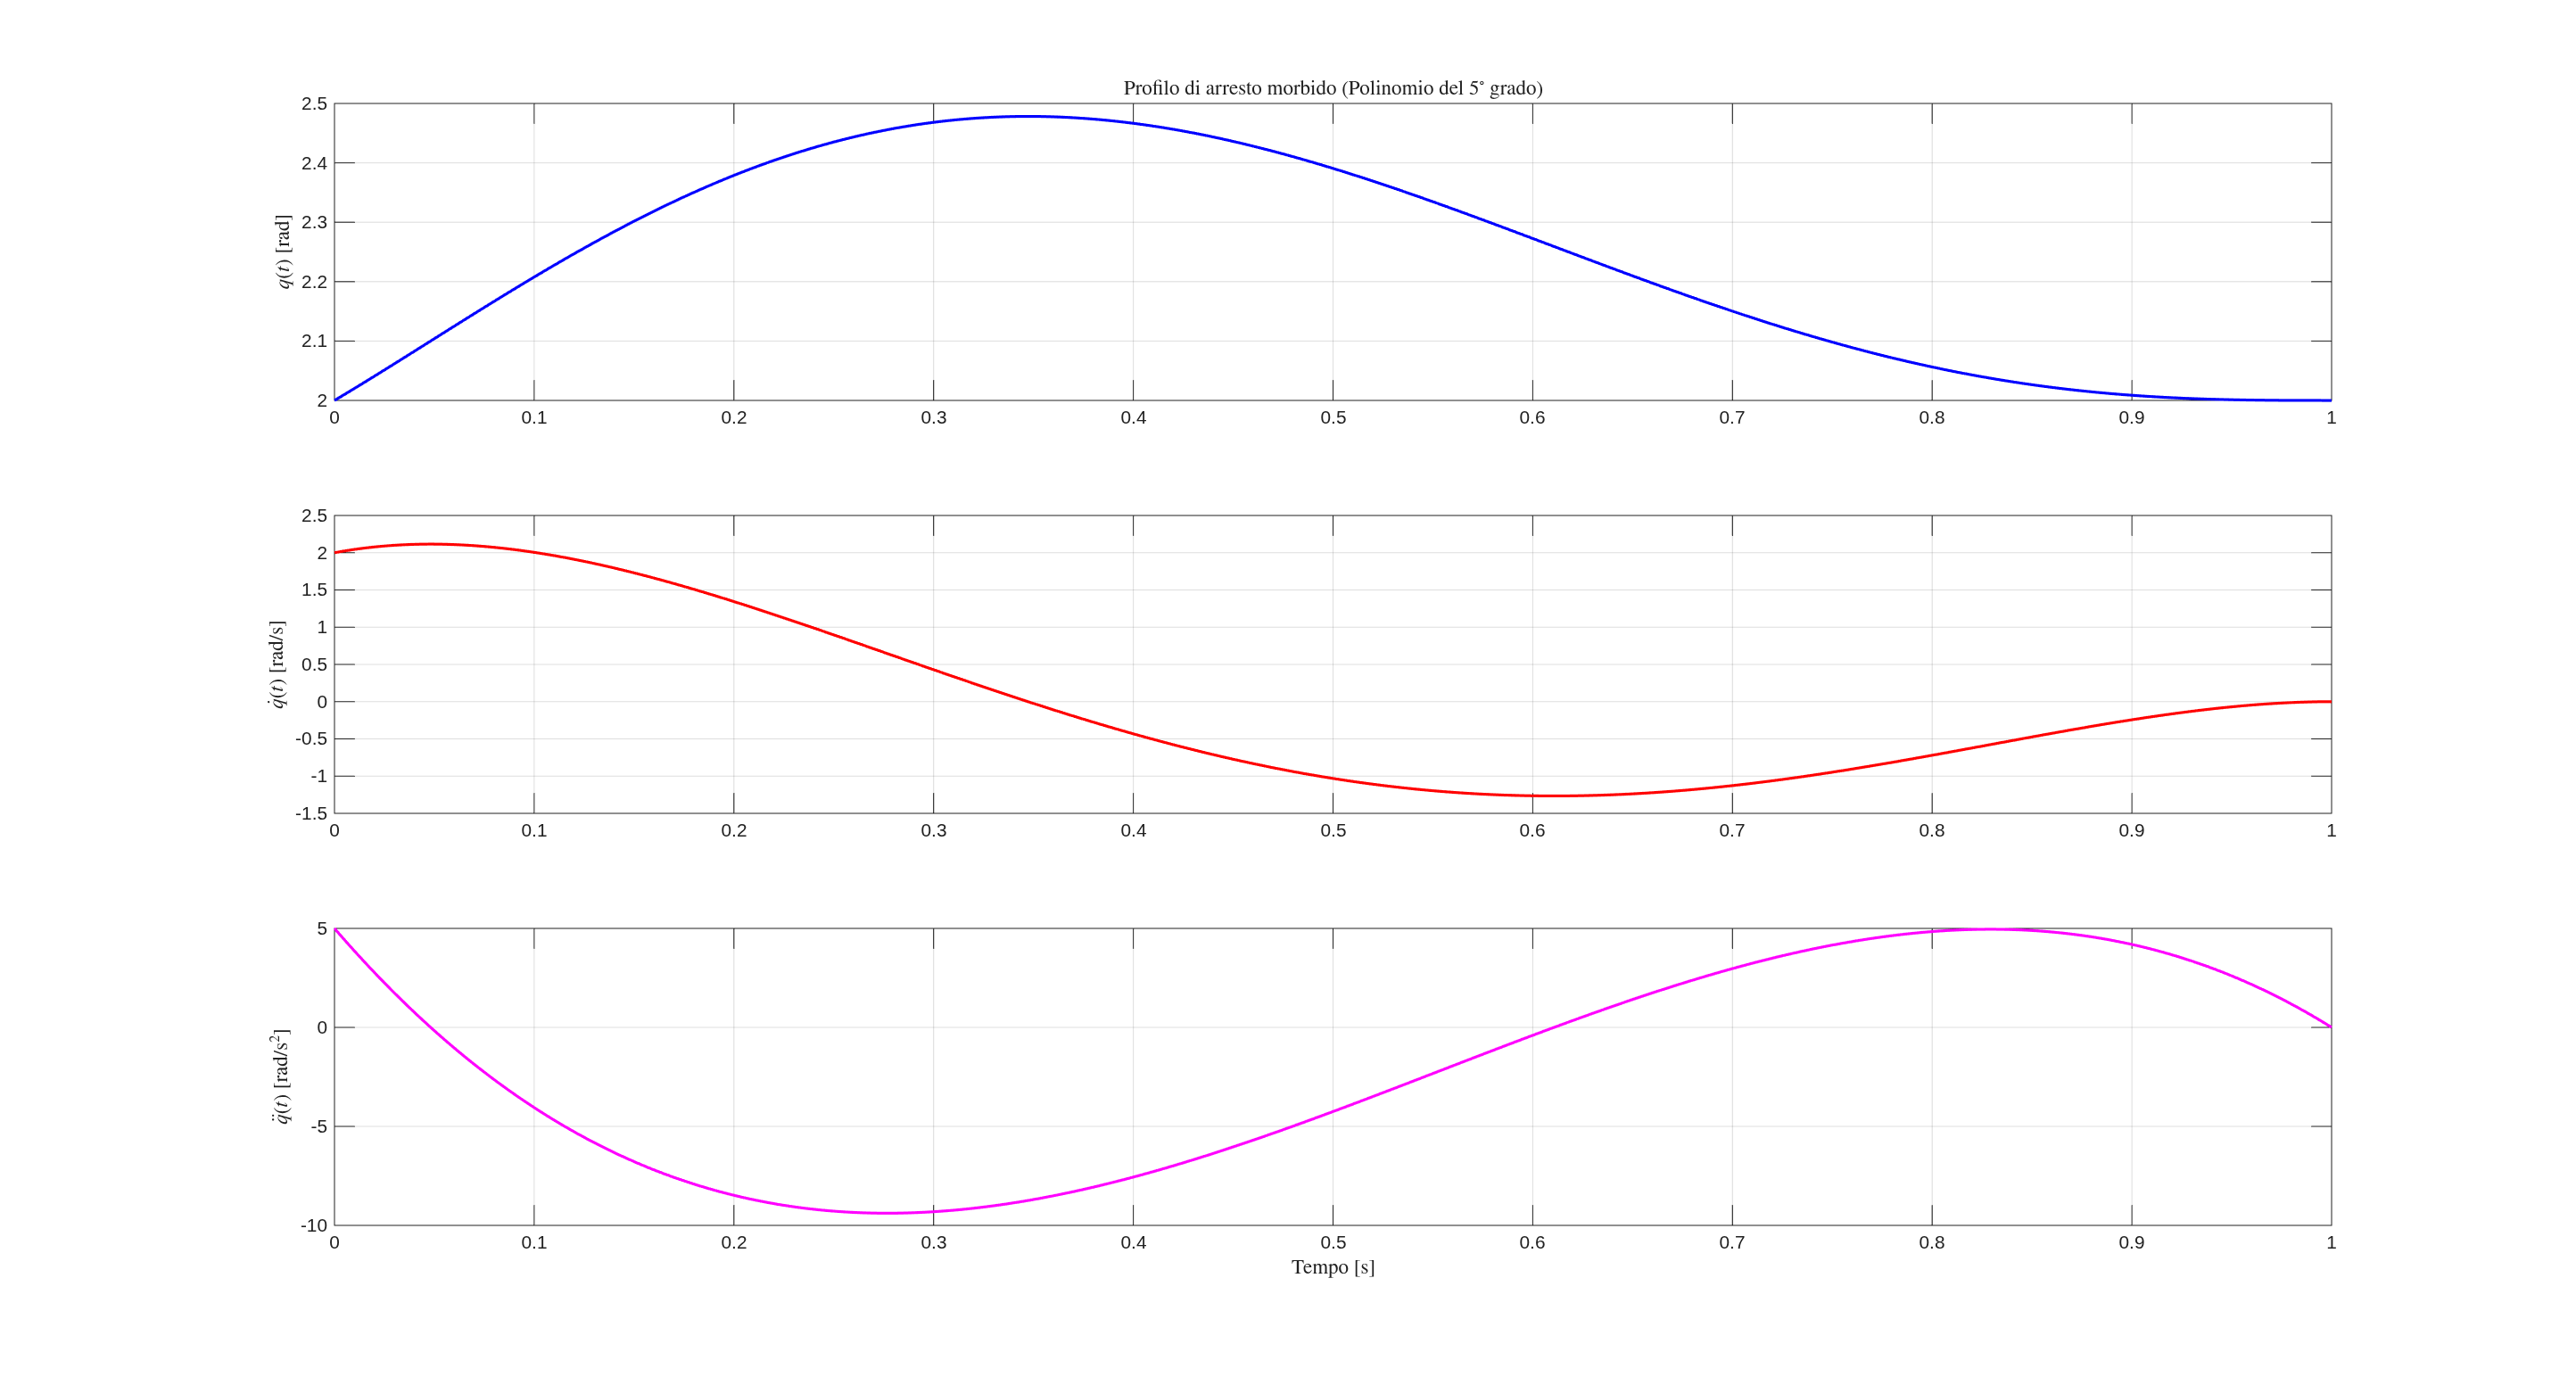
\includegraphics[width=1\linewidth]{figure_tesi/arresto_morbido.png}
    \caption{Profili temporali di posizione $q(t)$, velocità $\dot{q}(t)$ e accelerazione $\ddot{q}(t)$ durante la manovra di arresto morbido con polinomio quintico.}
    \label{fig:arresto_morbido}
\end{figure}

Si noti che in questa formulazione si impone che la posizione obiettivo di arresto al tempo $t_f$ corrisponda alla posizione $q_{i,j}$ registrata all'istante di innesco della frenata, come si può notare dalla Figura~\ref{fig:arresto_morbido}. Sarà compito della pianificazione polinomiale quintica garantire la continuità e la sicurezza dell'arresto lungo l'intervallo $T_{\text{stop}}$, gestendo la transizione a partire dalla velocità iniziale non nulla $\dot{q}_{i,j} \neq 0$.



\subsection{Formulazione dell'ottimizzazione e vincoli dinamici}
\label{subsec:optimization_problem}
La determinazione del tempo di arresto minimo $T_{\text{stop}}$ viene formulata come un problema di ottimizzazione vincolata ad ogni passo di controllo \cite{Scalera2024, Scalera2022}:
\begin{equation}
    \min_{T_{\text{stop}}} \quad w_0 T_{\text{stop}} + w_1 \left|T_{\text{stop}}-T_{\text{stop,prev}} \right|
    \label{eq:funzione_costo}
\end{equation}
dove $w_0, w_1 > 0$ sono pesi di ponderazione e $T_{\text{stop,prev}}$ rappresenta la soluzione computata al ciclo precedente. La presenza del termine penalizzante $|T_{\text{stop}} - T_{\text{stop,prev}}|$ introduce un'azione di regolarizzazione, garantendo continuità temporale nelle dimensioni delle capsule ed evitando variazioni brusche dell'area di ingombro tra iterazioni successive.

L'ottimizzazione dell'equazione \ref{eq:funzione_costo} è soggetta al rispetto stringente dei limiti cinematici e dinamici del manipolatore per tutta la durata della frenata, $\forall t \in [t_i, t_f]$:
\begin{align}
    |\dot{q}_j(t)| &\le \dot{q}_{j,\max} \quad &\forall j=1, \dots, 7 \label{eq:vel_lim}\\
    |\ddot{q}_j(t)| &\le \ddot{q}_{j,\max} \quad &\forall j=1, \dots, 7 \label{eq:acc_lim}\\
    |\dddot{q}_j(t)| &\le \dddot{q}_{j,\max} \quad &\forall j = 1, \dots, 7 \label{eq:jerk_lim}\\
    |\tau_j(t)| &\le \tau_{j,\max} \quad &\forall j = 1, \dots, 7 \label{eq:torque_lim}\\
    |\dot{\tau}_j(t)| &\le \dot{\tau}_{j,\max} \quad &\forall j = 1, \dots, 7 \label{eq:dtorque_lim}
\end{align}

Il vettore delle coppie ai giunti $\tau(t) \in \mathbb{R}^n$ è legato allo stato cinematico attraverso il modello dinamico inverso dell'equazione di Lagrange:
\begin{equation}
    \tau(t) = M(q)\ddot{q} + C(q, \dot{q})\dot{q} + g(q)
\end{equation}
In cui $M(q) \in \mathbb{R}^{7 \times 7}$ rappresenta la matrice d'inerzia, $C(q, \dot{q} \in \mathbb{R}^{7 \times 7}$ include i termini centripeti e di Coriolis e $g(q) \in \mathbb{R}^7$ è il vettore delle forze di gravità.

Attraverso la soluzione dell'equazione \eqref{eq:funzione_costo}, il sistema calcola il tempo di frenata minimo ammissibile. Ciò consente di modellare capsule di sicurezza protettive con l'ingombro spaziale strettamente necessario, massimizzando lo spazio di 
lavoro condiviso ed evitando arresti non necessari durante l'esecuzione del task.

\section{Secondo approccio: capsule \textit{soft}}

Per minimizzare le interruzioni operative e garantire una continuità di servizio nello spazio di lavoro collaborativo, il secondo approccio introduce l'impiego di capsule \textit{soft}. Rispetto ai volumi di ingombro impiegati per la gestione degli arresti di sicurezza, queste capsule presentano dimensioni in generale maggiori e definiscono una fascia di interazione dinamica tra il robot e l'operatore umano. In questo scenario, un'eventuale intersezione tra le capsule del manipolatore e le \textit{Sphere Swept Lines} (SSL) associate all'operatore non determina un arresto immediato del sistema, ma innesca una strategia di evasione attiva basata sul ricalcolo in tempo reale della traiettoria del task\cite{Qyrani2026}.

\subsection{Confronto tra capsule \textit{hard} e \textit{soft}}

Per armonizzare i requisiti di produttività e sicurezza, questa architettura prevede l'adozione simultanea di due set concentrici di capsule:

\begin{itemize}
    \item \textbf{Capsule \textit{hard}:} presentano dimensioni prossime al volume d'ingombro fisico del manipolatore e svolgono una funzione puramente protettiva. Come descritto nella Sezione~\ref{sec:primo_approccio}, una loro eventuale intersezione con le SSL dell'operatore indica una violazione dei margini minimi di sicurezza e comporta l'attivazione immediata dell'arresto con traiettoria di frenata morbida a profilo quintico.
    \item \textbf{Capsule \textit{soft}:} possiedono un raggio maggiorato e sono vincolate alla struttura dei bracci robotici. Esse definiscono una zona di pre-allarme dinamica: la misura del grado di penetrazione o sovrapposizione con le SSL dell'operatore non arresta il robot, ma viene impiegata per sintesi e calcolo della forza repulsiva virtuale responsabile della deviazione di traiettoria.
\end{itemize}

L'azione combinata dei due set garantisce che il robot cerchi prima di evitare attivamente l'operatore tramite le capsule \textit{soft} e, solo nel caso in cui l'evasione non sia sufficiente a prevenire la violazione delle capsule \textit{hard}, intervenga la procedura di arresto sicuro.

\subsection{Controllo di ammettenza per l'evasione dinamica}

Il ricalcolo della traiettoria in tempo reale si fonda sull'implementazione di uno schema di controllo di ammettenza nello spazio cartesiano. Nell'ambito del controllo dell'interazione, la letteratura distingue tra approcci d'impedenza e d'ammettenza in base alle relazioni di causalità adottate:
\begin{itemize}
    \item \textbf{Controllo d'impedenza (Causalità Moto $\rightarrow$ Forza):} accetta un errore/deviazione di posizione come ingresso e calcola la forza o coppia di reazione da applicare al robot.
    \item \textbf{Controllo d'ammettenza (Causalità Forza $\rightarrow$ Moto):} misura o sintetizza una forza esterna come ingresso e la converte in un riferimento di moto (posizione, velocità e accelerazione).
\end{itemize}

Poiché i controllori industriali standard e le API di basso livello del robot sono tipicamente ottimizzati con anelli interni di posizione e velocità ad elevata rigidezza, il controllo d'ammettenza risulta l'approccio ideale. Esso agisce come un filtro dinamico esterno che genera un nuovo riferimento cinematico inviabile direttamente ai servocomandi di giunto del manipolatore.

\subsubsection{Sintesi della forza repulsiva e dinamica dell'ammettenza}

Nel nostro scenario di evasione non si ha un contatto fisico reale con l'operatore; la vicinanza dell'uomo all'interno della capsula \textit{soft} viene tradotta in una forza repulsiva virtuale $\boldsymbol{F}_{\text{rep}} \in \mathbb{R}^6$. Tale forza ha modulo proporzionale alla profondità di penetrazione all'interno della fascia \textit{soft} ed è diretta lungo la retta di minima distanza tra i segmenti geometrici.

La forza virtuale $\boldsymbol{F}_{\text{rep}}$ viene fornita in ingresso al modello dell'ammettenza cartesiana, che modella l'interfaccia di contatto come un sistema meccanico equivalente di tipo massa-molla-smorzatore:
\begin{equation}
\boldsymbol{M}_d \big(\ddot{\boldsymbol{x}}_r - \ddot{\boldsymbol{x}}_d\big) + \boldsymbol{D}_d \big(\dot{\boldsymbol{x}}_r - \dot{\boldsymbol{x}}_d\big) + \boldsymbol{K}_d \big(\boldsymbol{x}_r - \boldsymbol{x}_d\big) = \boldsymbol{F}_{\text{rep}}
\label{eq:admittance_dynamics}
\end{equation}

dove:
\begin{itemize}
    \item $\boldsymbol{x}_d, \dot{\boldsymbol{x}}_d, \ddot{\boldsymbol{x}}_d \in \mathbb{R}^6$ indicano le grandezze cartesiane desiderate (posizione, velocità, accelerazione) pianificate dal task nominale. Lo spazio $\mathbb{R}^6$ viene adottato per descrivere completamente i 6 gradi di libertà del manipolatore nello spazio operativo, includendo sia le 3 componenti traslazionali sia le 3 componenti rotazionali dell'organo terminale;
    \item $\boldsymbol{x}_r, \dot{\boldsymbol{x}}_r, \ddot{\boldsymbol{x}}_r \in \mathbb{R}^6$ rappresentano lo stato di riferimento modificato che viene calcolato online;
    \item $\boldsymbol{M}_d, \boldsymbol{D}_d, \boldsymbol{K}_d \in \mathbb{R}^{6 \times 6}$ costituiscono le matrici simmetriche e definite positive di massa, smorzamento e rigidezza virtuali desiderate.
\end{itemize}

\subsubsection{Calcolo online della posizione modificata}

L'equazione~(\ref{eq:admittance_dynamics}) descrive un sistema differenziale del secondo ordine. Esplicitando il termine di accelerazione modificata $\ddot{\boldsymbol{x}}_r$, si ottiene:
\begin{equation}
\ddot{\boldsymbol{x}}_r = \ddot{\boldsymbol{x}}_d + M_d^{-1} \Big( \boldsymbol{F}_{\text{rep}} - D_d \big(\dot{\boldsymbol{x}}_r - \dot{\boldsymbol{x}}_d\big) - K_d \big(\boldsymbol{x}_r - \boldsymbol{x}_d\big) \Big)
\end{equation}

Attraverso schemi di integrazione numerica in tempo reale (es. Eulero o Runge-Kutta al ciclo di controllo a 1 kHz), questa accelerazione viene integrata passo-passo per ricavare la velocità $\dot{\boldsymbol{x}}_r(t)$ e infine la nuova posizione cartesiana di riferimento $\boldsymbol{x}_r(t)$. 

Il comportamento del robot durante l'evasione è governato dai parametri della matrice virtuale:
\begin{itemize}
    \item Azione della massa ($\boldsymbol{M}_d$): filtra i picchi improvvisi della forza repulsiva, garantendo accelerazioni fluide ed evitando scatti bruschi.
    \item Azione dello smorzamento ($\boldsymbol{D}_d$): dissipa l'energia del sistema virtuale e previene l'insorgere di oscillazioni indesiderate durante l'allontanamento dall'operatore.
    \item Azione della rigidezza ($\boldsymbol{K}_d$): agisce come un richiamo elastico verso la traiettoria nominale $\boldsymbol{x}_d(t)$. Nel momento in cui l'operatore esce dalla capsula \textit{soft}, la forza repulsiva $\boldsymbol{F}_{\text{rep}}$ si annulla e il termine $K_d$ riporta gradualmente e in modo fluido il robot sul percorso pianificato originario.
\end{itemize}

Infine, la posizione cartesiana modificata $\boldsymbol{x}_r(t)$ viene convertita nelle corrispondenti variabili di giunto $\boldsymbol{q}_r(t)$ tramite cinematica inversa differenziale (sfruttando lo Jacobiano analitico o geometrico del robot) e inviata all'anello di controllo di posizione interno.

